\documentclass[sigconf]{acmart}

\usepackage{booktabs} % For formal tables
\usepackage{graphicx}
\usepackage{balance}  % for  \balance command ON LAST PAGE  (only there!)
\usepackage{amssymb}
\usepackage{graphicx}
\usepackage{float}
\usepackage{subfigure}
\usepackage{mathtools}
\usepackage{eurosym}

\usepackage{pgfplots}
\usepackage{url}
\usepackage{enumitem}
\usepackage[linesnumbered,ruled]{algorithm2e}
\usepackage[export]{adjustbox}
\usepackage{xspace}
\usepackage{breqn}

% Copyright
%\setcopyright{none}
%\setcopyright{acmcopyright}
%\setcopyright{acmlicensed}
\setcopyright{rightsretained}
%\setcopyright{usgov}
%\setcopyright{usgovmixed}
%\setcopyright{cagov}
%\setcopyright{cagovmixed}


% DOI
\acmDOI{10.475/XXX_X}

% ISBN
\acmISBN{XXX-XXX-XX-XXX/10/18}

%Conference
\acmConference[CIKM'18]{ACM International Conference on Information and Knowledge Management}{October 2018}{
  Lingotto, Turin Italy}
\acmYear{2018}
\copyrightyear{2018}


\acmArticle{4}
\acmPrice{15.00}

% These commands are optional
%\acmBooktitle{Transactions of the ACM Woodstock conference}
\editor{Rakesh Agrawal}
\editor{Andrei Broder}
\editor{Mohammed Zaki}


\begin{document}
\title{Exploring interesting dense regions on spatial data.}
%\titlenote{Produces the permission block, and
%  copyright information}
%\subtitle{Extended Abstract}
%\subtitlenote{The full version of the author's guide is available as
%  \texttt{acmart.pdf} document}


%\author{Behrooz Omidvar-Tehrani}
%\affiliation{%
 % \institution{University of Grenoble Alpes (France)}
%}
%\email{behrooz.omidvar-tehrani@univ-grenoble-alpes.fr}

%\author{Pl\'acido A. Souza Neto}
%\affiliation{%
 % \institution{Federal Institute of Rio Grande do Norte (Brazil)}
%}
%\email{placido.neto@ifrn.edu.br}


%\author{Francisco B. Silva J\'unior}
%\affiliation{%
%\institution{Federal Institute of Rio Grande do Norte (Brazil)}
%}
%\email{bento.francisco@academico.ifrn.edu.br}	

%\author{Felipe F. Pontes}
%\affiliation{%
%\institution{Federal Institute of Rio Grande do Norte (Brazil)}
%}
%\email{freire.pontes@academico.ifrn.edu.br}


%\author{Tiago Oliveira Lisboa}
%\affiliation{%
% \institution{Federal Institute of Rio Grande do Norte (Brazil)}
% }
%\email{tiago.oliveira@academico.ifrn.edu.br}



% The default list of authors is too long for headers.
%\renewcommand{\shortauthors}{B. Trovato et al.}


\begin{abstract}

The large size of spatial data hinders its effective analysis for discovering insights. Analysts require to obtain only few options (so-called ``highlights'') to focus on. In this paper, we define, formalize and analyse the concept of interesting dense regions (IDR) in order to find possible preferred regions to the analyst. The objective is to obtain one or several regions in which the analyst has expressed her implicit feedback. Our proposal consider a polygon-based abstraction layer for captured interactions. Using these interesting dense regions, we highlight points to guide the analysis process. We also analyse its efficiency and effectiveness through a realistic example.
\end{abstract}

%
% The code below should be generated by the tool at
% http://dl.acm.org/ccs.cfm
% Please copy and paste the code instead of the example below.
%
%\begin{CCSXML}
%<ccs2012>
 %<concept>
  %<concept_id>10010520.10010553.10010562</concept_id>
  %<concept_desc>Computer systems organization~Embedded systems</concept_desc>
  %<concept_significance>500</concept_significance>
 %</concept>
 %<concept>
  %<concept_id>10010520.10010575.10010755</concept_id>
  %<concept_desc>Computer systems organization~Redundancy</concept_desc>
  %<concept_significance>300</concept_significance>
 %</concept>
 %<concept>
  %<concept_id>10010520.10010553.10010554</concept_id>
  %<concept_desc>Computer systems organization~Robotics</concept_desc>
  %<concept_significance>100</concept_significance>
 %</concept>
 %<concept>
 % <concept_id>10003033.10003083.10003095</concept_id>
  %<concept_desc>Networks~Network reliability</concept_desc>
  %<concept_significance>100</concept_significance>
 %</concept>
%</ccs2012>
%\end{CCSXML}

%\ccsdesc[500]{Computer systems organization~Embedded systems}
%\ccsdesc[300]{Computer systems organization~Redundancy}
%\ccsdesc{Computer systems organization~Robotics}
%\ccsdesc[100]{Networks~Network reliability}


\keywords{Dense regions, highlight, IDR, spatial data, implicit feedback.}


\maketitle

%\newpage
\section{Introduction}
Nowadays, there has been a meteoric rise in the generation of spatial datasets in various fields of science, such as transportation, lodging services and social science. As each record in spatial data represents an activity in a precise geographical location, analyzing such data enables discoveries grounded on facts. Analysts are often interested to observe spatial patterns and trends to improve their decision making process. Spatial data analysis has various applications such as smart city management, disaster management and autonomous transport \cite{RoddickEHPS04,Telang:2012}.

\vspace{2pt}
Typically, spatial data analysis begins with an imprecise question in the mind of the analyst, i.e., {\em exploratory analysis}. The analyst requires to go through several trail-and-error iterations to improve her understanding of the spatial data and gain insights. Each iteration involves visualizing a subset of data on geographical maps using an  off-the-shelf product (e.g., Tableau\footnote{\it http://www.tableau.com}, Exhibit\footnote{\it http://www.simile-widgets.org/exhibit/}, Spotfire\footnote{\it http://spotfire.tibco.com}) where the analyst can investigate on different parts of the visualization by zooming in/out and panning on the map. 

\vspace{3pt}
Spatial data are often voluminous. Hence the focus in the literature of spatial data analysis is on ``efficiency'', i.e., enabling fluid means of navigation in spatial data to facilitate the exploratory analysis. The common approach is to design pre-computed indexes which enable efficient retrieval of spatial data (e.g., \cite{lins2013nanocubes}). However, there has been fewer attention to the ``value'' derived from spatial data. Despite the huge progress on the efficiency front, an analyst may easily get lost in the plethora of geographical points due to two following reasons.

\vspace{3pt}
\noindent $\blacksquare$ In an exploratory context, the analyst doesn't know apriori what to investigate next.

\vspace{2pt}
\noindent $\blacksquare$ Moreover, she may easily get distracted and miss interesting points by visual clutter caused by huge point overlaps.

\vspace{3pt}
The main drawback of the traditional analysis model is that the analyst has a {\em passive role} in the process. In other words, the analyst's feedback (i.e., her likes and dislikes) is ignored and only the input query (i.e., her explicit request) is served. In case feedback is incorporated, the process can be more directed towards analyst's interests where her partial needs can be served earlier in the process. In this paper, we advocate for a ``guidance layer'' on top of the raw visualization of spatial data to enable analysts know {\em ``what to see next''}. This guidance should be a function of analyst feedback: the system should recommend options similar to what the analyst has already appreciated. 
% Hence, feedback capturing lies at the core of such guidance system.

\vspace{2pt}
Various approaches in the literature propose methodologies to incorporate analyst's feedback in the exploration process of spatial data. Typically, feedback is considered as a function which is triggered by any analyst's action on the map. The action can be ``selecting a point'', ``moving to a region'', ``asking for more details'', etc. The function then updates a ``profile vector'' which keeps tracks of analyst's interests. The updated content in the profile vector enables the guidance functionality. For instance, if the analyst shows interest in a point which describes a house with balcony, this choice of amenity will reflect her profile to prioritize other houses with balcony in future iterations.

\vspace{2pt}
Feedback is often expressed {\em explicitly}, i.e., the analyst clicks on a point and mentions if she likes or dislikes the point \cite{kamat2014distributed,Omidvar-Tehrani:2015,omidvar2017geoguide}. In \cite{omidvar2017geoguide}, we proposed an interactive approach to exploit such feedback for enabling a more insightful exploration of spatial data. However, there are several cases that the feedback is expressed {\em implicitly}, i.e., the analyst does not explicitly click on a point, but there exists correlations with other signals captured from the analyst which provide hint on her interest. For instance, it is often the case in spatial data analysis that analysts look at some regions of interest but do not provide an explicit feedback. Another example is frequent mouse moves around a region which is a good indicator of the analyst's potential interest in the points in that region. Implicit feedbacks are more challenging to capture and hence less investigated in the literature. The following example describes a use case of implicit feedbacks. This will be our running example which we follow thoughout the paper.

\vspace{2pt}
\noindent {\bf Example.} {\em Ben\'icio is planning to live in Paris for a season. He decides to rent a home-stay from Airbnb website\footnote{\it http://www.airbnb.com}. He likes to discover the city, hence he is open to any type of lodging in any region with an interest to stay in the center of Paris. The website returns 1500 different locations. As he has no other preferences, an exhaustive investigation needs scanning each location independently which is nearly infeasible. While he is scanning few first options, he shows interest in the region of Trocadero (where the Eiffel tower is located in) but he forgets or doesn't feel necessary to click a point there. An ideal system should capture this implicit feedback in order to short-list a small subset of locations that Ben\'icio should consider as high priority}.

\vspace{2pt}
The above example shows in practice that implicit feedback capturing is crucial in the context of spatial data analysis. While text-boxes, combo-boxes and other input elements are available in analyzing other types of data, the only interaction means between the analyst and a spatial data analysis system is a geographical map spanned on the whole screen. In this context, a point can be easily remained out of sight and missed.

\vspace{2pt}
In this paper, we present an approach called {\sc GeoPoly} whose aim is to capture and analyze implicit feedback of analysts in spatial data analysis. Without loss of generality, we focus on ``mouse moves'' as the implicit feedback received from the analyst. Mouse moves are the most common way that analysts interact with geographical maps~\cite{Chen:2001}. It is shown in \cite{Arapakis:2014} that mouse gestures have a strong correlation with ``user engagement''. Intuitively, a point gets a higher weight in the analyst's profile if the mouse cursor moves around it frequently.  However, our approach can be easily extended to other types of inputs such gaze tracking, leap motions, etc.

% \cite{Robertson2007}  affirms that temporal change in spatial patterns are increasingly common in geographical analysis. This work explore an approach to the spatialtemporal analysis of polygons that are spatially distinct and experience discrete changes though time. It presents challenges considering changes of regions (polygons) during the time. Works like \cite{Ester:1996} and  \cite{Birant:2007} present solutions for clustering spatialtemporal data. These solutions are relevant to define regions by each cluster that contains important informations for the user. 

% \vspace{3pt}
% Discovering patterns and provide tendencies in spatial data applications may improve insights for planning and decision making for smart city solutions. Many systems and datasets consider space information.  In this way, find spatial preferences can offer interactive and guidance solutions.  For example,  when users look for a house or hotel to spend a season, they consider one or more regions of their preference. These regions are intrinsic to each user, or user group. However, when navigating the application, the user also considers regions that seem interesting, for different reasons, such as the priority of some tourist spot, restaurants, clubs, security, etc. Thus, capturing region preferences over time can help to guide the user to find better places.
 
% \vspace{3pt}
% Given a dataset of spatial points and from the mouse tracking movements by the user, our approach generates a set of highlighted regions based on its preferences. Each region is related with a subset of highlighted points which are illustrated using visual variables such as size and color intensity. The regions are also highlighted.

\vspace{2pt}
The outline of the paper is the following. Section \ref{sec:datamodel} describes our data model. In Section \ref{sec:problem}, we formally define our problem. Then in Section \ref{sec:algo}, we present our solution and its algorithmic details. Section  \ref{sec:exp} reports our experiments on the framework. We review the related work in Section \ref{sec:rel}. Last, we conclude in Section \ref{sec:conc}.

\section{Introduction}



Spatial data are often voluminous. Hence the focus in the literature of spatial data analysis is on ``efficiency'', i.e., enabling fluid means of navigation in spatial data to facilitate the exploratory analysis. The common approach is to design pre-computed indexes which enable efficient retrieval of spatial data (e.g., \cite{lins2013nanocubes}). However, there has been fewer attention to the ``value'' derived from spatial data. Despite the huge progress on the efficiency front, an analyst may easily get lost in the plethora of geographical points due to two following reasons.

\vspace{3pt}
\noindent $\blacksquare$ In an exploratory context, the analyst doesn't know apriori what to investigate next.

\vspace{2pt}
\noindent $\blacksquare$ Moreover, she may easily get distracted and miss interesting points by visual clutter caused by huge point overlaps.

\vspace{3pt}
The main drawback of the traditional analysis model is that the analyst has a {\em passive role} in the process. In other words, the analyst's feedback (i.e., her likes and dislikes) is ignored and only the input query (i.e., her explicit request) is served. In case feedback is incorporated, the process can be more directed towards analyst's interests where her partial needs can be served earlier in the process. In this paper, we advocate for a ``guidance layer'' on top of the raw visualization of spatial data to enable analysts know {\em ``what to see next''}. This guidance should be a function of analyst feedback: the system should recommend options similar to what the analyst has already appreciated. 
 
In this paper, we present an approach to explore Interesting Dense Regions (IDRs)  whose aim is to capture and analyze implicit feedback of analysts in spatial data analysis. Without loss of generality, we focus on ``mouse moves'' as the implicit feedback received from the analyst. Mouse moves are the most common way that analysts interact with geographical maps~\cite{Chen:2001}.  However, our approach can be easily extended to other types of inputs such gaze tracking, leap motions, etc.

% K-DBSCAN with the main focus of identifying clusters of points with similar spatial density.  K-DBSCAN lies in finding arbitrary shaped clusters in variable density regions. Moreover, it can also discover clusters with overlapping spatial regions, but differing density levels.
 
 
\section{Interesting Dense Regions}


An Interesting Dense Region (\textit{IDR}) is a region with high possibility to have a set of point that may be interesting to the analyst. An IDR is captured and defined by processing user feedbacks. Unlike the literature which mainly focuses on explicit feedback (where the analyst should clearly reflect her likes and dislikes), we investigate on implicit feedback. There are different ways to capture implicit feedbacks: (\textit{i}) During spatial data analysis, it is often the case that analysts look at some regions of interest but forget to provide an explicit feedback. We call this latent signal, gaze. It shown in [5] that gaze has a strong correlation with ``user attention''. The signal can be captured by tracking eye movements \citep{arapakis2014user}; (\textit{ii}) To address privacy issues of web-cam exploitation for gaze tracking, we consider an alternative option of tracking the mouse cursor. It is shown in \cite{arapakis2014understanding} that mouse gestures have a strong correlation with ``user engagement''. Intuitively, a point receives a positive feedback if the cursor moves around it frequently. (\textit{iii}) In most spatial datasets, there is a profile page dedicated to each point.  We consider the amount of time that the analyst spends in a page as an implicit feedback. For instance, if the analyst spends few minutes in a page for an apartment with balcony in center of Paris, this counts as positive feedback for this type of apartment. So, the objective of IDR's definition is to obtain one or several regions in which the analyst has expressed her implicit feedback. 

There are two observations for such regions definition:

\vspace{2pt}
\noindent $\blacksquare$ {\bf Observation 1.} We believe that a region appeals more interesting to the analyst if it is denser, i.e., the analyst moves her mouse in that region several times.

\vspace{2pt}
\noindent $\blacksquare$ {\bf Observation 2.} It is possible that the analyst moves her mouse everywhere in the map. This should not signify that everywhere in the map has the same significance.

We consider two different layers on a geographical map: ``spatial layer'' and ``interaction layer''. The spatial layer contains points from a spatial database $\mathcal{P}$. The interaction layer contains mouse move points $\mathcal{M}$.

Our proposal algorithm mines a set of mouse move points $\mathcal{M}$ in the interaction layer to discover one or several Interesting Dense Regions, in which most analyst's interactions occur. Then it matches the spatial points $\mathcal{P}$ with IDRs  in order to find points inside each region. The attributes of resulting points will be exploited to update a analyst's feedback vector. The updated vector $F$ will then be used to find $k$ highlights. These steps ensure that the final highlights reflect analyst's implicit interests. 

Following our observations, we propose Algorithm \ref{algo:dense} for mining IDRs. We add points to $\mathcal{M}$ only every $200ms$ to prevent adding redundant points.  Following Observation 1 and in order to mine the recurring behavior of the analyst, the algorithm begins by partitioning the set $\mathcal{M}$ into $g$ fixed-length consecutive segments $\mathcal{M}_0$ to $\mathcal{M}_g$. The first segment starts at time zero (where the system started), and the last segment ends at $t_c$, i.e., the current time. Following Observation 2, we then find dense clusters in each segment of $\mathcal{M}$ using a variant of DB-SCAN~\cite{Ester:1996} approach. Finally, we return intersections among those clusters as IDRs.




\begin{algorithm}[t]
\DontPrintSemicolon
\KwIn{Current time $t_c$, mouse move points $\mathcal{M}$}
\KwOut{IDRs $\mathcal{S}$}
$\mathcal{S} \gets \emptyset$\;
$g \gets ${\em number of time segments}\;
\For{$i \in [0,g]$}
{
       $\mathcal{M}_i \gets \{m = \langle x,y,t \rangle | (\frac{t_c}{g} \times i) \leq t \leq (\frac{t_c}{g} \times (i+1))\}$\;
       $\mathcal{C}_i \gets \mathit{mine\_clusters}(\mathcal{M}_i)$\label{ln:mine}\;
       $\mathcal{O}_i \gets \mathit{find\_ploygons}(\mathcal{C}_i)$\label{ln:poly}\;
}
\lFor{$\mathcal{O}_i, \mathcal{O}_j$ where $i,j \in [0,g]$ and $i \neq j$}
{
       $\mathcal{S}.\mathit{append}(\mathit{intersect}(\mathcal{O}_i, \mathcal{O}_j))$
}
\Return{$\mathcal{S}$}\; 
\caption{Find Interesting Dense Regions (IDRs)}
\label{algo:dense}
\end{algorithm}


\vspace{2pt}
For clustering points in each time segment (i.e., line \ref{ln:mine} of Algorithm~\ref{algo:dense}), we use ST-DBSCAN~\cite{Birant:2007}, a space-aware variant of DB-SCAN for clustering points based on density. For each subset of mouse move points $\mathcal{M}_i$, $i \in [0,g]$, ST-DBSCAN begins with a random point $m_0 \in \mathcal{M}_i$ and collects all density-reachable points from $m_0$ using a distance metric. As mouse move points are the 2-dimensional pixel space (i.e., the display), we choose euclidean distance as the distance metric. If $m_0$ turns out to be a core object, a cluster will be generated. Otherwise, if $m_0$ is a border object, no point is density-reachable from $m_0$ and the algorithm picks another random point in $\mathcal{M}_i$. The process is repeated until all of the points have been processed.

\vspace{2pt}
Once clusters are obtained for all subsets of $\mathcal{M}$, we find their intersections to locate recurring regions (line \ref{ln:poly}). To obtain intersections, we need to clearly define the spatial boundaries of each cluster. Hence for each cluster, we discover its corresponding polygon that covers the points inside. For this aim, we employ Quickhull algorithm, a quicksort-style method which computes the convex hull for a given set of points in a 2D plane~\cite{Barber:1996}.


\section{Case Study and Experiments}

This section describes an example to guide the experiments made over the proposal presented in this paper. The following use case describes a scenario of implicit feedbacks. 


\begin{figure*}[t]
\centering
   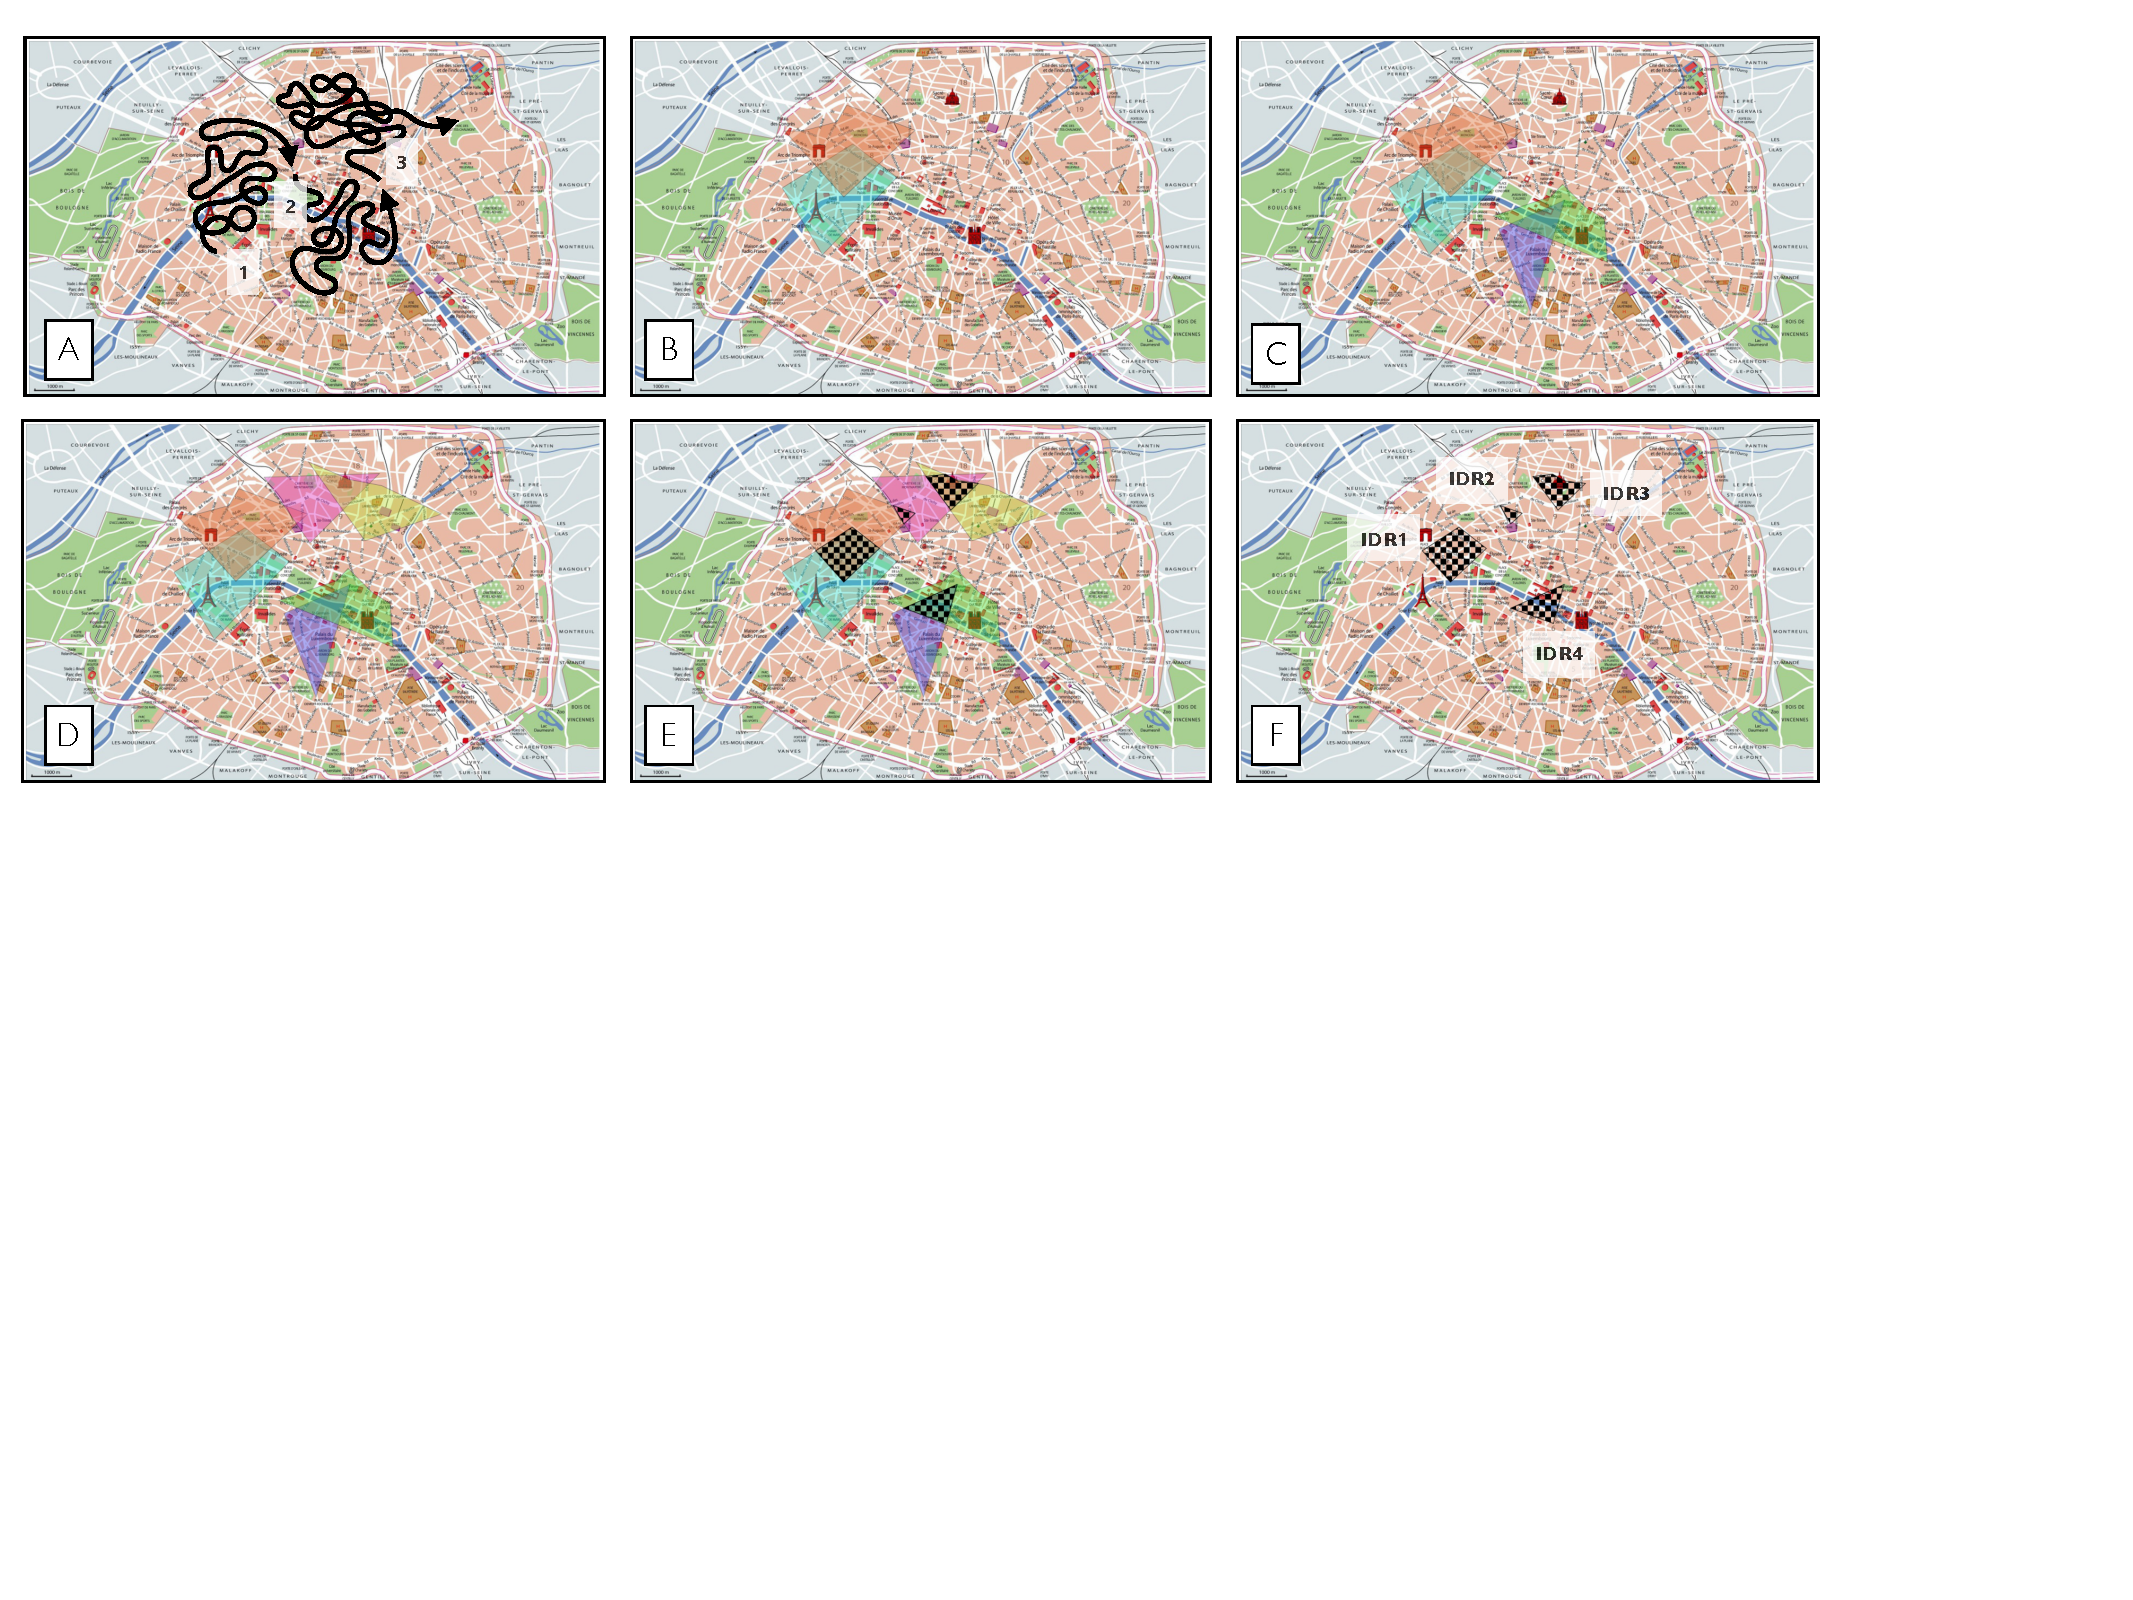
\includegraphics[width=\textwidth]{imgs/regions}
  \caption{The process of finding IDRs - Paris city.}
  \label{fig:regions}
\end{figure*}



\begin{figure}[t]
\centering
   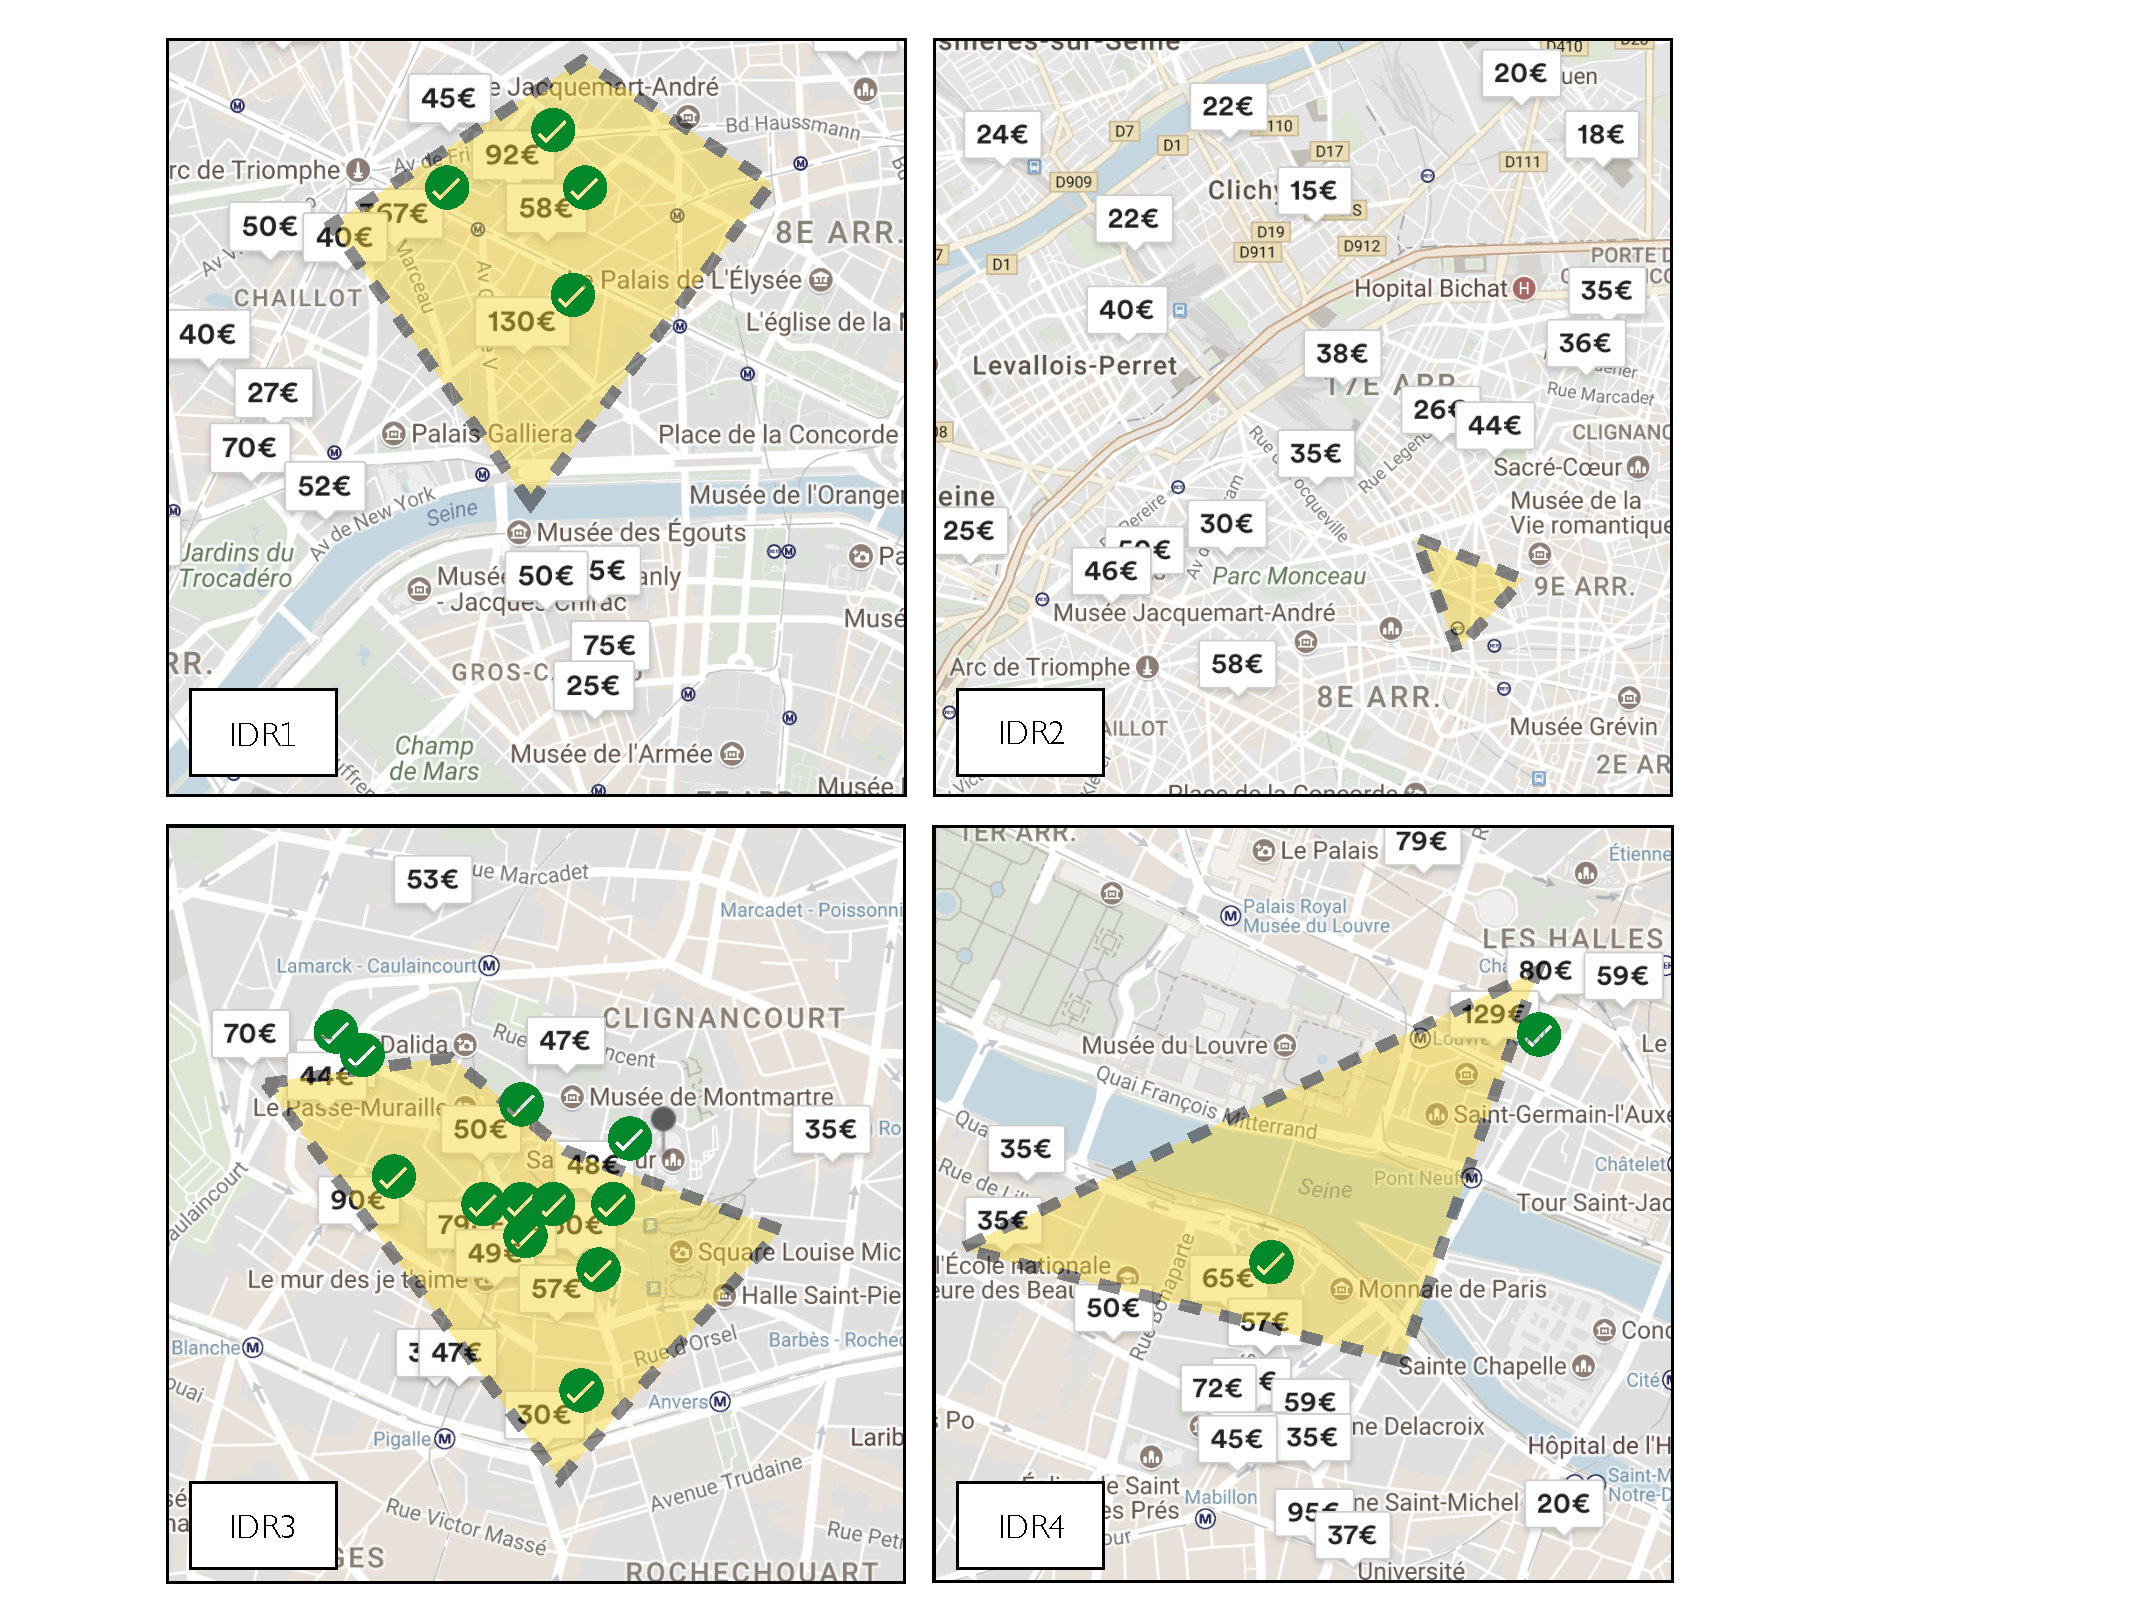
\includegraphics[width=\columnwidth]{imgs/match}
  \caption{Matching points for IDRs.}
  \label{fig:match}
\end{figure}

\vspace{2pt}
\noindent {\bf Example.} {\em Lucas is planning to pass some days in Paris, France. He loves French culture and language, and pass some days in a nice city would be delighted to him.  He decides to rent a home-stay from Airbnb website\footnote{\it http://www.airbnb.com}. He likes to discover the city, hence he is open to any type of lodging in any region with an interest to stay in the city center. The website returns 1500 different locations. As he has no other preferences, an exhaustive investigation needs scanning each location independently which is nearly infeasible. While he is scanning few first options, he shows interest in the region of \textit{Champ de Mars} (close to Eiffel Tower), but he forgets or doesn't feel necessary to click a point there. An ideal system should capture this implicit feedback in order to short-list a small subset of locations that Lucas should consider as high priority}.

We describe the process of finding IDRs in an example. Figure \ref{fig:regions} shows the steps that Lucas follows in our running example to explore home-stays in Paris. Figure \ref{fig:regions}.A shows mouse movements of Lucas in different time stages. In this example, we consider $g = 3$ and capture Lucas feedback in three different time segments (progressing from Figures \ref{fig:regions}.B to \ref{fig:regions}.D). It shows that Lucas started his search around Eiffel Tower and Arc de Triomphe (Figure \ref{fig:regions}.B) and gradually showed interest in south (Figure \ref{fig:regions}.C) and north (Figure \ref{fig:regions}.D) as well. All intersections between those clusters are discovered (hatching regions in Figure \ref{fig:regions}.E) which will constitute the set of IDRs (Figure \ref{fig:regions}.F), i.e., IDR1 to IDR4.


In the Airbnb dataset points are home-stays which are shown with their nightly price on the map. We observe (Figure \ref{fig:match}) that there exist many matching points with IDR3 and absolutely no matching point for IDR2. For IDR4, although there exist many home-stays below the region, we never check their containment, as they belong to a Quadtree cell which doesn't intersect with the IDR. 

Considering the described example we perform a first set of few experiments to validate its efficiency and effectiveness. In the interest of space, we only present a glimpse of our experiments here. More will be discussed in an extended version. 

\vspace{2pt}
First off, we validate the ``usability'' of our proposal. For this aim, we design a user study with some participants who are all students of Computer Science. Some of them are ``novice'' users who don't know the location, and some are ``experts''. Participants should fulfill a task. For each participant, we report a variant of time-to-insight measure, i.e., how long the participants interact with the frameworks before fulfilling the task. Evidently, less number of interactions is preferred as it means that the participant can reach insights faster. Then we measure the time to execute the task.


\vspace{2pt}
On the Airbnb dataset of Paris with 1,000 points, we define two different tasks: {\em T1: ``finding a point in a requested location''} (e.g., find a home-stay in the ``\textit{Champ de Mars}'' area), and {\em T2: ``finding a point with a requested profile''} (e.g., find a cheap home-stay.) Participants may also begin their navigation either from {\em I1: ``close to the goal''} or {\em I2: ``far from the goal''}. 


\begin{table}[h]
\centering
\caption{``Novice'' and ``Experts'' - Interactions (in seconds)}
\label{tbl:novice}
\begin{tabular}{c|c|c|c|c|}
\cline{2-5}
                                       	& \textbf{T1/I1} 	& \textbf{T2/I1} 	& \textbf{T1/I2}	& \textbf{T2/I2}	\\ \hline
\multicolumn{1}{|c|}{Novices} 				& 1.99            	& 2.38	          	& 2.00              & 2.48              \\ \hline
\multicolumn{1}{|c|}{Experts} 				& 1.72            	& 2.09	          	& 1.70              & 2.14              \\ \hline
\end{tabular}
\end{table}


\vspace{2pt}
Participants benefit from information highlighting based on their implicit feedback. Table \ref{tbl:novice} reports the time for the interactions to find what they are looking for, novice and expert participants, respectively. We observe that on average the system spends $2.067$ seconds to return a defined goal. This shows that implicit feedback capturing is an effective mechanism which helps analysts to reach their goals faster.

\vspace{2pt}
Expert participants need $0.35$ (seconds) fewer interactions on average. Interestingly, starting points, i.e., {\em I1} and {\em I2}, do not have a huge impact on number of steps. It is potentially due to the diversity component which provides distinct options and can quickly guide analyst towards their region of interest. We also observe that the task {\em T2} is an easier task than {\em T1}. This is potentially due to  where the analyst can request options similar to what she has already observed and greedily move to her preferred regions.

\vspace{4pt}
We also perform a second set of experiments considering 2 different datasets~\footnote{Airbnb and Yelp datasets with spatial points of Paris city}.  

.... [Experiment Description] .....\\
.... [Experiment Description] .....\\
.... [Experiment Description] .....\\
.... [Experiment Description] .....\\

\begin{table}[h]
\centering
\caption{Airbnb dataset - Paris city}
\label{tbl:airbnb}
\begin{tabular}{|c|c|c|c|c|}
\cline{1-5}
\textbf{n. points}  & \textbf{regions} 	& \textbf{IDRs} 	& \textbf{points in IDRs}	& \textbf{\%  points}	\\ \hline
\multicolumn{1}{|c|}{100} 				& 11.35            	& 10.05	          	& 29.40             & 29.40\%            
 \\ \hline
\multicolumn{1}{|c|}{1000} 				& 10.75          	& 6.75	          	& 11.70              & 1.17\%              \\ \hline
\multicolumn{1}{|c|}{2000} 				& 7.37           	& 3.63         	& 5.63             & 0.003\%              \\ \hline
\multicolumn{1}{|c|}{4000} 				& 10.30           	& 10.15	          	& 53.15              & 1.33\%              \\ \hline

\end{tabular}
\end{table}

.... [Experiment Description] .....\\
.... [Experiment Description] .....\\
.... [Experiment Description] .....\\
.... [Experiment Description] .....\\

\begin{table}[h]
\centering
\caption{Yelp dataset - Paris city}
\label{tbl:airbnb}
\begin{tabular}{|c|c|c|c|c|}
\cline{1-5}
\textbf{n. points}  & \textbf{regions} 	& \textbf{IDRs} 	& \textbf{points in IDRs}	& \textbf{\%  points}	\\ \hline
\multicolumn{1}{|c|}{100} 				& 14.90            	& 7.55	          	& 28.30             & 28.30\%            
 \\ \hline
\multicolumn{1}{|c|}{1000} 				& 13.90         	& 10.00	          	& 149.55             & 14.96\%              \\ \hline
\multicolumn{1}{|c|}{2000} 				& 11.05         	& 9.80         	& 111.05             & 5.55\%              \\ \hline
\multicolumn{1}{|c|}{4000} 				& 10.45          	& 8.55	          	& 145.7              & 3.64\%              \\ \hline

\end{tabular}
\end{table}

.... [Experiment Description] .....\\
.... [Experiment Description] .....\\
.... [Experiment Description] .....\\
.... [Experiment Description] .....\\
.... [Experiment Description] .....\\
.... [Experiment Description] .....\\
.... [Experiment Description] .....\\
.... [Experiment Description] .....\\

\section{Conclusions}

In this paper, we propose to explore Interesting Dense Regions (\textit{IDRs}) of spatial information highlighting using implicit feedback. The implicit feedbacks are captured from mouse movements of the analyst over the geographical map. We formulate and formalize a novel polygon-based capturing algorithm which returns few highlights (regions) in line with analyst's implicit preferences. 

\vspace{2pt}
We consider some directions of improvement for this work. We are interested to incorporate an ``explainability'' component  which can describe causalities behind preferences. For instance, we are interested to find seasonal patterns to see why the preferences of analysts change from place to place during various seasons of the year. Another direction is to incorporate ``Query by Visualization'' approaches, where analysts can specify their intents alongside their implicit preferences, directly on the map \cite{siddiqui2016effortless}.

\bibliographystyle{ACM-Reference-Format}
\bibliography{main}

\end{document}
